% !TeX root = main.tex

\chapter{Finite Impulse Response (FIR) Filters}
\glsresetall
\label{chapter:fir}

\section{Overview}
Finite Impulse Response (FIR) filters are commonplace in digital signal processing (DSP) applications -- they are perhaps the most widely used operation in this domain. They are well suited for hardware implementation since they can be implemented as a highly optimized architecture. A key property is that they are a linear transform on contiguous elements of a signal. This maps well to data structures (e.g., FIFOs or tap delay lines) that can be implemented efficiently in hardware. In general, streaming applications tend to map well to FPGAs, e.g., most of the examples that we present throughout the book have some sort of streaming behavior. 

Two fundamental uses for a filter are signal restoration and signal separation. Signal separation is perhaps the more common use case: here one tries to isolate the input signal into different parts. Typically, we think of these as different frequency ranges, e.g., we may want perform a low pass filter in order remove high frequencies that are not of interest. Or we may wish to perform a band pass filter to determine the presence of a particular frequency in order to demodulate it, e.g., for isolating tones during frequency shift keying demodulation.  Signal restoration relates to removing noise and other common distortion artifacts that may have been introduced into the signal, e.g., as data is being transmitted across the wireless channel. This includes smoothing the signal and removing the DC component.

Digital FIR filters often deal with a discrete signal generated by sampling a continuous signal. The most familiar sampling is performed in time, i.e., the values from a signal are taken at discrete instances. These are most often sampled at regular intervals. For instance, we might sample the voltage across an antenna at a regular interval with an analog-to-digital converter. Alternatively we might sample the current created by a photo-diode to determine the light intensity.  Alternatively, samples may be taken in space.  For instance, we might sample the value of different locations in an image sensor consisting of an array of photo-diodes to create a digital image.  More in-depth descriptions of signals and sampling can be found in \cite{lee2011signalsandsystems}.

The format of the data in a sample changes depending upon the application. Digital communications often uses complex numbers (in-phase and quadrature or I/Q values) to represent a sample. Later in this chapter we will describe how to design a complex FIR filter to handle such data. In image processing we often think of a pixel as a sample. A pixel can have multiple fields, e.g., red, green, and blue (RGB) color channels.  We may wish to filter each of these channels in a different way again depending upon the application.

The goal of this chapter is to provide a basic understanding of the process of taking an algorithm and creating a good hardware design using high-level synthesis. The first step in this process is always to have a deep understanding of the algorithm itself. This allows us to make design optimizations like code restructuring much more easily. The next section provides an understanding of the FIR filter theory and computation. The remainder of the chapter introduces various HLS optimizations on the FIR filter. These are meant to provide an overview of these optimizations. Each of them will described in more depth in subsequent chapters. 

\section{Background}

The output signal of a filter given an impulse input signal is its \term{impulse response}. The impulse response of a linear, time invariant filter contains the complete information about the filter. As the name implies, the impulse response of an FIR filter (a restricted type of linear, time invariant filter) is finite, i.e., it is always zero far away from zero.  Given the impulse response of an FIR filter, we can compute the output signal for any input signal through the process of \term{convolution}.  This process combines samples of the impulse response (also called \term{coefficients} or \term{taps}) with samples of the input signal to compute samples of the output signal.  The output of filter can be computed in other ways (for instance, in the frequency domain), but for the purposes of this chapter we will focus on computing in the time domain.

The convolution of an N-tap FIR filter with coefficients $h[]$ with an input signal $x[]$ is described by the general difference equation:
\begin{equation}
y[i] =  \displaystyle\sum\limits_{j=0}^{N-1} h[j] \cdot x[i-j]
\end{equation}
Note that to compute a single value of the output of an N-tap filter requires N multiplies and N-1 additions.

%\note{Talk about moving average filters to introduce FIR}
\term{Moving average filters} are a simple form of lowpass FIR filter where all the coefficients are identical and sum to one. For instance in the case of the three point moving filter, the coefficients are $h = [\frac{1}{3}, \frac{1}{3}, \frac{1}{3}]$.  It is also called a \term{box car filter} due to the shape of its convolution kernel.  Alternatively, you can think of a moving average filter as taking the average of several adjacent samples of the input signal and averaging them together. We can see that this equivalence by substituting $1/N$ for $h[j]$ in the convolution equation above and rearranging to arrive at the familiar equation for an average of $N$ elements:
\begin{equation}
y[i] = \frac{1}{N} \displaystyle\sum\limits_{j=0}^{N} x[i-j]
\end{equation}

Each sample in the output signal can be computer by the above equation using $N-1$ additions and one final multiplication by $1/N$.  Even the final multiplication can often be regrouped and merged with other operations.  As a result, moving average filters are simpler to compute than a general FIR filter.  Specifically, when $N = 3$ we perform this operation to calculate $y[12]$:
\begin{equation}
y[12] = \frac{1}{3} \cdot (x[12] + x[11] + x[10])
\end{equation}
This filter is \term{causal}, meaning that the output is a function of no future values of the input. It is possible and common to change this, for example, so that the average is centered on the current sample, i.e., $y[12] = \frac{1}{3} \cdot (x[11] + x[12] + x[13])$. While fundamentally causality is an important property for system analysis, it is less important for a hardware implementation as a finite non-causal filter can be made causal with buffering and/or reindexing of the data.

Moving average filters can be used to smooth out a signal, for example to remove random (mostly high frequency) noise.   As the number of taps $N$ gets larger, we average over a larger number of samples, and we correspondingly must perform more computations. For a moving average filter, larger values of $N$ correspond to reducing the bandwidth of the output signal. In essence, it is acting like a low pass filter (though not a very optimal one). Intuitively, this should make sense. As we average over larger and larger number of samples, we are eliminating higher frequency variations in the input signal. That is, ``smoothing'' is equivalent to reducing higher frequencies. The moving average filter is optimal for reducing white noise while keeping the sharpest step response, i.e., it creates the lowest noise for a given edge sharpness.
\note{The previous paragraph has alot of concepts.  Can we add a reference here?}

Note that in general, filter coefficients can be crafted to create many different kinds of filters: low pass, high pass, band pass, etc.. In general, a larger value of number of taps provides more degrees of freedom when designing a filter, generally resulting in filters with better characteristics. There is substantial amount of literature devoted to generating filter coefficients with particular characteristics for a given application. When implementing a filter, the actual values of these coefficients are largely irrelevant and we can ignore how the coefficients themselves were arrived at.  However, as we saw with the moving average filter, the structure of the filter, or the particular coefficients can have a large impact on the number of operations that need to be performed.  For instance, symmetric filters have multiple taps with exactly the same value which can be grouped to reduce the number of multiplications.  In other cases, it is possible to convert the multiplication by a known constant filter coefficient into shift and add operations \cite{kastner2010arithmetic}. In that case, the values of the coefficients can drastically change the performance and area of the filter implementation \cite{mirzaei2007fpga}. But we will ignore that for the time being, and focus on generating architectures that have constant coefficients, but do not take advantage of the values of the constants.
%\note{Make sure that I'm using the term ``tap'' correctly. I believe that tap is equal to N-1 coefficients for some odd reason.}

\section{Base FIR Architecture}
\label{sec:base_fir}

Consider the code for an 11 tap FIR filter in Figure \ref{fig:fir11_initial}. The function takes two arguments, an input sample \lstinline{x}, and the output sample \lstinline{y}. This function must be called multiple times to compute an entire output signal, since each time that we execute the function we provide one input sample and receive one output sample. This code is convenient for modeling a streaming architecture, since we can call it as many times as needed as more data becomes available.

\begin{figure}
\lstinputlisting{examples/fir11_initial.c}
\caption{A functionally correct, but highly unoptimized, implementation of an 11 tap FIR filter. }
\label{fig:fir11_initial}
\end{figure}

The coefficients for the filter are stored in the \lstinline{c[]} array declared inside of the function. These are statically defined constants. Note that the coefficients are symmetric. i.e., they are mirrored around the center value \lstinline{c[5] = 500}. Many FIR filter have this type of symmetry. We could take advantage of it in order to reduce the amount of storage that is required for the \lstinline{c[]} array.

The code uses \lstinline{typedef} for the different variables. While this is not necessary, it is convenient for changing the types of data. As we discuss later, bit width optimization -- specifically setting the number of integer and fraction bits for each variable -- can provide significant benefits in terms of performance and area.  

\begin{exercise}
Rewrite the code so that it takes advantage of the symmetry found in the coefficients. That is, change \lstinline{c[]} so that it has six elements (\lstinline{c[0]} through \lstinline{c[5]}). What changes are necessary in the rest of the code? How does this effect the number of resources? How does it change the performance?
\end{exercise}

The code is written as a streaming function. It receives one sample at a time, and therefore it must store the previous samples. Since this is an 11 tap filter, we must keep the previous 10 samples. This is the purpose of the \lstinline{shift_reg[]} array. This array is declared \lstinline{static} since the data must be persistent across multiple calls to the function. 

The \lstinline{for} loop is doing two fundamental tasks in each iteration. First, it performs the multiply and accumulate operation on the input samples (the current input sample \lstinline{x} and the previous input samples stored in \lstinline{shift_reg[]}). Each iteration of the loop performs a multiplication of one of the constants with one of the sample, and stores the running sum in the variable \lstinline{acc}. The loop is also shifting values through \lstinline{shift_array}, which works as a FIFO. It stores the input sample \lstinline{x} into  \lstinline{shift_array[0]}, and moves the previous elements ``up'' through the \lstinline{shift_array}:

\begin{padbox}{.5\textwidth}
\noindent\lstinline{shift_array[10] = shift_array[9]} \\
\lstinline{shift_array[9]  =  shift_array[8]} \\
\lstinline{shift_array[8]  =  shift_array[7]} \\
$\cdots$ \\
\lstinline{shift_array[2]  =  shift_array[1]} \\
\lstinline{shift_array[1]  =  shift_array[0]} \\
\lstinline{shift_array[0]  =  x} \\
\end{padbox}
\begin{aside}
The label \lstinline{Shift_Accum_Loop:} is not necessary. However it can be useful for debugging. The \VHLS tool adds these labels into the views of the code. 
\end{aside}

After the for loop completes, the \lstinline{acc} variable has the complete result of the convolution of the input samples with the FIR coefficient array. The final result is written into the function argument \lstinline{y} which acts as the output port from this \lstinline{fir} function. This completes the streaming process for computing one output value of an FIR.

This function does not provide an efficient implementation of a FIR filter. It is largely sequential, and employs a significant amount of unnecessary control logic. The following sections describe a number of different optimizations that improve its performance.

\section{Calculating Performance}
\label{sec:fir-performance}
%\note{This discussion may be better in Chapter 1.}

Before we get into the optimizations, it is necessary to define precise metrics. When deriving the performance of a design, it is important to carefully state the metric. For instance, there are many different ways of specifying how ``fast'' your design runs. For example, you could say that it operates at $X$ bits/second. Or that it can perform $Y$ operations/sec. Other common performance metrics specifically for FIR filters talk about the number of filter operations/second. Yet another metric is multiply accumulate operations: MACs/second. Each of these are related to one another, in some manner, but when comparing different implementations it is important to compare apples to apples. For example, directly comparing one design using bits/second to another using filter operations/second can be misleading; fully understanding the relative benefits of the designs requires that we compare them using the same metric. And this may require additional information, e.g., going from filter operations/second to bits/second requires information about the size of the input and output data. 

All of the aforementioned metrics use seconds. High-level synthesis tools talk about the designs in terms of number of cycles, and the frequency of the clock. The frequency is inversely proportional to the time it takes to complete one clock cycle. Using them both gives us the amount of time in seconds to perform some operation. The number of cycles and the clock frequency are both important: a design that takes one cycle, but with a very low frequency is not necessary better than another design that takes 10 clock cycles but operates at a much higher frequency. 

The clock frequency is a complicated function that the \VHLS tool attempts to optimize alongside the number of cycles. Note that it is possible to specify a target frequency to the \VHLS tool. This is done using the \lstinline{create_clock} tcl command.  For example, the command \lstinline{create_clock -period 5} directs the tool to target a clock period of 5 ns and equivalently a clock frequency of 200 MHz.  Note that this is only a target clock frequency only and primarily affects how much operation chaining is performed by the tool.  After generating RTL, the \VHLS tool provides an initial timing estimate relative to this clock target.  However, some uncertainty in the performance of the circuit remains which is only resolved once the design is fully place and routed.

While achieving higher frequencies are often critical for reaching higher performance, increasing the target clock frequency  is not necessarily optimal in terms of an overall system. Lower frequencies give more leeway for the tool to combine multiple dependent operations in a single cycle, a process called \term{operation chaining}. This can sometimes allow higher performance by enabling improved logic synthesis optimizations and increasing the amount of code that can fit in a device. Improved operation chaining can also improve (i.e., lower) the initiation interval of pipelines with recurrences.   In general providing a constrained, but not over constrained target clock latency is a good option. Something in the range of $5 - 10$ ns is typically a good starting option. Once you optimize your design, you can vary the clock period and observe the results. We will describe operation chaining in more detail in the next section.

Because \VHLS deals with clock frequency estimates, it does include some margin to account for the fact that there is some error in the estimate.  The goal of this margin is to ensure enough timing slack in the design that the generated RTL can be successfully placed and routed.  This margin can be directly controlled using the \lstinline{set_clock_uncertainty} TCL command.  Note that this command only affects the HLS generated RTL and is different from the concept of clock uncertainty in RTL-level timing constraints.  Timing constraints generated by \VHLS for the RTL implementation flow are solely based on the target clock period.

It is also necessary to put the task that you are performing in context with the performance metric that you are calculating. In our example, each execution of the \lstinline{fir} function results in one output sample. But we are performing $N = 11$ multiply accumulate operations for each execution of \lstinline{fir}. Therefore, if your metric of interest is MACs/second, you should calculate the task latency for \lstinline{fir} in terms of seconds, and then divide this by $11$ to get the time that it takes to perform the equivalent of one MAC operation. 

Calculating performance becomes even more complicated as we perform pipelining and other optimizations. In this case, it is important to understand the difference between task interval and task latency. It is a good time to refresh your understanding of these two metrics of performance. This was discussed in Chapter \ref{sec:designOptimization}. And we will continue to discuss how different optimizations effect different performance metrics.

\section{Operation Chaining}
\label{sec:fir-chaining}

\term{Operation chaining} is an important optimization that the \VHLS performs in order to optimize the final design. It is not something that a designer has much control over, but it is important that the designer understands how this works especially with respect to performance. Consider the multiply accumulate operation that is done in a FIR filter tap. Assume that the \lstinline{add} operation takes 2 ns to complete, and a \lstinline{multiply} operation takes 3 ns. If we set the clock period to 1 ns (or equivalently a clock frequency of 1 GHz), then it would take 5 cycles for the MAC operation to complete. This is depicted in Figure \ref{fig:mac} a). The \lstinline{multiply} operation is executed over 3 cycles, and the \lstinline{add} operation is executed across 2 cycles. The total time for the MAC operation is 5 cycles $\times$ 1 ns per cycle $=$ 5 ns. Thus we can perform 1/5 ns $=$ 200 million MACs/second. 

\begin{figure}
\centering
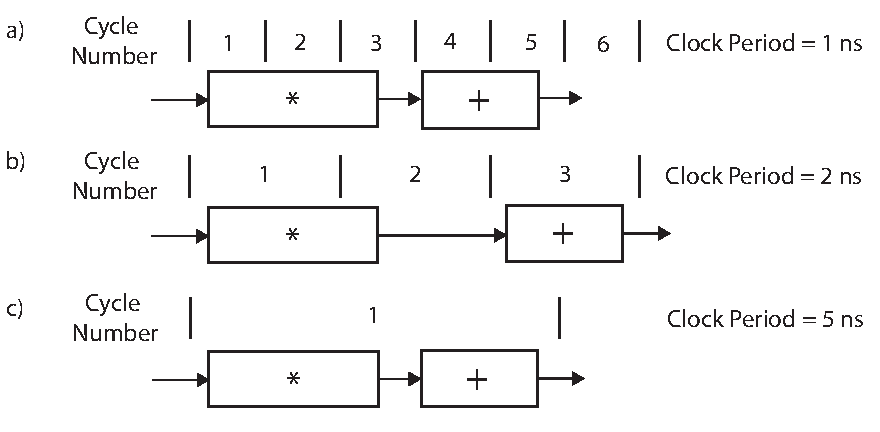
\includegraphics[width=5.5in]{images/mac}
\caption{The performance of multiply accumulate operation changes depending upon the target clock period. Assume the \lstinline{multiply} operation takes 3 ns and \lstinline{add} operation takes 2 ns. Part a) has a clock period of 1 ns, and one MAC operation takes 5 cycles. Thus the performance is 200 million MACs/sec. Part b) has a clock period of 2 ns, and the MAC takes 3 cycles resulting in approximately 167 million MACs/sec.  Part c) has a clock period of 5 ns. By using operation chaining, a MAC operation takes 1 cycle for a clock period of 200 million MACs/sec. }
\label{fig:mac}
\end{figure}

If we increase the clock period to 2 ns, the \lstinline{multiply} operation now spans over two cycles, and the \lstinline{add} operation must wait until cycle 3 to start. It can complete in one cycle. Thus the MAC operation requires 3 cycles, so 6 ns total to complete. This allows us to perform approximately 167 million MACs/second. This result is lower than the previous result with a clock period of 1 ns. This can be explained by the ``dead time'' in cycle 2 where no operation is being performed.

However, it is not always true that increasing the clock period results in worse performance. For example, if we set the clock period to 5 ns, we can perform both the \lstinline{multiply} and \lstinline{add} operation in the same cycle using operation chaining. This is shown in Figure \ref{fig:mac} c). Thus the MAC operation takes 1 cycle where each cycle is 5 ns, so we can perform 200 million MACs/second. This is the same performance as Figure \ref{fig:mac} a) where the clock period is faster (1 ns). 

So far we have performed chaining of only two operations in one cycle. It is possible to chain multiple operations in one cycle. For example, if the clock period is 10 ns, we could perform 5 \lstinline{add} operations in a sequential manner. Or we could do two sequential MAC operations. 

It should start to become apparent that the clock period plays an important role in how the \VHLS tool optimizes the design. This becomes even more complicated with all of the other optimizations that the \VHLS tool performs. It is not that important to fully understand the entire process of the \VHLS tool. This is especially true since the tool is constantly being improved with each new release. However, it is important to have a good idea about how the tool may work. This will allow you to better comprehend the results, and even allow you to write more optimized code. 

Although the \VHLS can generate different different hardware for different target clock periods, overall performance optimization and determining the optimal target clock period still requires some creativity on the part of the user. For the most part, we advocate sticking within a small subset of clock periods. For example, in the projects we suggest that you set the clock period to 10 ns and focus on understanding how other optimizations, such as pipelining, can be used to create different architectures. This 100 MHz clock frequency is relatively easy to achieve, yet it is provides a good first order result. It is certainly possible to create designs that run at a faster clock rate.  200 MHz and faster designs are possible but often require more careful balance between clock frequency targets and other optimization goals.  You can change the target clock period and observe the differences in the performance. Unfortunately, there is no good rule to pick the optimal frequency. 

\begin{exercise}
Vary the clock period for the base FIR architecture (Figure \ref{fig:fir11_initial}) from 10 ns to 1 ns in increments of 1 ns. Which clock period provides the best performance? Which gives the best area? Why do you think this is the case? Do you see any trends? 
\end{exercise}

\section{Code Hoisting}

The \lstinline{if/else} statement inside of the \lstinline{for} loop is inefficient.  For every control structure in the code, the \VHLS tool creates logical hardware that checks if the condition is met, which is executed in every iteration of the loop. Furthermore, this conditional structure limits the execution of the statements in either the \lstinline{if} or \lstinline{else} branches; these statements can only be executed after the \lstinline{if} condition statement is resolved.

The \lstinline{if} statement checks when \lstinline{x == 0}, which happens only on the last iteration. Therefore, the statements within the \lstinline{if} branch can be ``hoisted'' out of the loop. That is we can execute these statements after the loop ends, and then remove the \lstinline{if/else} control flow in the loop. Finally, we must change the loop bounds from executing the ``0th'' iteration. This transform is shown in Figure \ref{fig:fir11_ifelse}. This shows just the changes that are required to the \lstinline{for} loop. 

\begin{figure}
\lstinputlisting{examples/fir11_ifelse.c}
\caption{ Removing the conditional statement from the \lstinline{for} loop creates a more efficient hardware implementation. }
\label{fig:fir11_ifelse}
\end{figure}

The end results is a much more compact implementation that is ripe for further loop optimizations, e.g., unrolling and pipelining. We discuss those optimizations later.

\begin{exercise}
Compare the implementations before and after the removal of the \lstinline{if/else} condition done through loop hoisting. What is the difference in performance? How do the number of resources change?
\end{exercise}

%Conditional statements are synthesized as complex control logic, and thus should be avoided if possible. In this case, we can get rid of the condition. In other cases ternary operation is useful.

\section{Loop Fission}

We are doing two fundamental operations within the \lstinline{for} loop. The first part shifts the data through the \lstinline{shift_reg} array. The second part performs the multiply and accumulate operations in order to calculate the output sample. \term{Loop fission} takes these two operations and implements each of them in their own loop. While it may not intuitively seem like a good idea, it allows us to perform optimizations separately on each loop. This can be advantageous especially in cases when the resulting optimizations on the split loops are different. 

\begin{figure}
\lstinputlisting{examples/fir11_partition.c}
\caption{ A code snippet corresponding to splitting the \lstinline{for} loop into two separate loops. }
\label{fig:fir11_partition}
\end{figure}


The code in Figure \ref{fig:fir11_partition} shows the result of manual loop fission optimization.  The code snippet splits the loop from Figure \ref{fig:fir11_ifelse} into two loops. Note the label names for the two loops. The first is \lstinline{TDL} and the second is \lstinline{MAC}. \term{Tapped delay line (TDL)} is a common DSP term for the FIFO operation; MAC is short-hand for ``multiply accumulate''.

\begin{exercise}
Compare the implementations before and after loop fission. What is the difference in performance? How do the number of resources change?
\end{exercise}

Loop fission alone often does not provide a more efficient hardware implementation. However, it allows each of the loops to be optimized independently, which could lead to better results than optimizing the single, original \lstinline{for} loop. The reverse is also true; merging two (or more) \lstinline{for} loops into one \lstinline{for} loop may yield the best results. This is highly dependent upon the application, which is true for most optimizations. In general, there is not a single `rule of thumb' for how to optimize your code. There are many tricks of the trade, and your mileage may vary. Thus, it is important to have many tricks at your disposal, and even better, have a deep understanding of how the optimizations work. Only then will you be able to create the best hardware implementation. Let us continue to learn some additional tricks...

\section{Loop Unrolling}
By default, the \VHLS tool synthesizes \lstinline{for} loops in a sequential manner. The tool creates a data path that implements one execution of the statements in the body of the loop. The data path executes sequentially for each iteration of the loop. This creates an area efficient architecture; however, it limits the ability to exploit parallelism that may be present across loop iterations. 

\term{Loop unrolling} replicates the body of the loop by some number of times (called the \term{factor}). And it reduces the number of iterations of the loop by the same factor. In the best case, when none of the statements in the loop depend upon any of the data generated in the previous iterations, this can substantially increase the available parallelism, and thus enables an architecture that runs much faster. 

The first \lstinline{for} loop (with the label \lstinline{TDL}) in Figure \ref{fig:fir11_partition} shifts the values up through the \lstinline{shift_reg} array. The loop iterates from largest value (\lstinline{N-1}) to the smallest value (\lstinline{i = 1}). By unrolling this loop, we can create a data path that executes a number of these shift operations in parallel. 

\begin{figure}
\lstinputlisting{examples/fir11_unrollTDL.c}
\caption{ Manually unrolling the \lstinline{TDL} loop in the \lstinline{fir11} function.  }
\label{fig:fir11_unrollTDL}
\end{figure}

Figure \ref{fig:fir11_unrollTDL} shows the result of unrolling the loop by a factor of two. This code replicates the loop body twice. Each iteration of the loop now performs two shift operations. Correspondingly, we must perform half of the number of iterations.

Note that there is an additional \lstinline{if} condition after the \lstinline{for} loop. This is required in the case when the loop does not have an even number of iterations. In this case, we must perform the last ``half'' iteration by itself. The code in the \lstinline{if} statement performs this last ``half'' iteration, i.e., moving the data from \lstinline{shift_reg[0]} into \lstinline{shift_reg[1]}.

Also note the effect of the loop unrolling on the \lstinline{for} loop header. The decrement operation changes from \lstinline{i--} to \lstinline{i=i-2}. This is due to the fact that we are doing two times the ``work'' in each iteration, thus we should decrement by 2 instead of 1.

Finally, the condition for terminating the \lstinline{for} loop changes from \lstinline{i > 0} to \lstinline{i > 1}. This is related to the fact that we should make sure that the ``last'' iteration can fully complete without causing an error. If the last iteration of the \lstinline{for} loop executes when \lstinline{i = 1}, then the second statement would try to read from \lstinline{shift_reg[-1]}. Rather than perform this illegal operation, we do the final shift in the \lstinline{if} statement after the \lstinline{for} loop. 

\begin{exercise}
Write the code corresponding to manually unrolling this \lstinline{TDL for} loop by a factor of three. How does this change the loop body? What changes are necessary to the loop header? Is the additional code in the \lstinline{if} statement after the \lstinline{for} loop still necessary? If so, how is it different?
\end{exercise}

Loop unrolling can increase the overall performance provided that we have the ability to execute some (or all) of the statements in parallel. In the unrolled code, each iteration requires that we read two values from the \lstinline{shift_reg} array; and we write two values to the same array. Thus, if we wish to execute both statements in parallel, we must be able to perform two read operations and two write operations from the \lstinline{shift_reg} array in the same cycle. 

Assume that we store the \lstinline{shift_reg} array in one BRAM, and that BRAM has two read ports and one write port. Thus we can perform two read operations in one cycle. But we must sequentialize the write operations across two consecutive cycles. 

There are ways to execute these two statements in one cycle. For example, we could store all of the values of the \lstinline{shift_reg} array in separate registers. It is possible to read and write to each individual register on every cycle. In this case, we can perform both of the statements in this unrolled \lstinline{for} loop in one cycle. You can tell the \VHLS tool to put all of the values in the \lstinline{shift_reg} array into registers using the directive \lstinline{#pragma HLS array_partition  variable=shift_reg complete}. This is an important optimization, thus we discuss the \lstinline{array_partition} directive in more detail later. 

A user can tell the \VHLS tool to automatically unroll the loop using the \lstinline{unroll} directive. To automatically perform the unrolling done manually in Figure \ref{fig:fir11_unrollTDL}, we should put the directive \lstinline{#pragma HLS unroll factor=2} into the body of the code, right after the \lstinline{for} loop header. While we can always manually perform loop unrolling, it is much easier to allow the tool to do it for us. It makes the code easier to read; and it will result in fewer coding errors. 

\begin{exercise}
Unroll the \lstinline{TDL for} loop automatically using the \lstinline{unroll} directive. As you increase the unroll factor, how does this change the number of resources (FFs, LUTs, BRAMs, DSP48s, etc.)? How does it effect the throughput? What happens when you use the \lstinline{array_partition} directive in conjunction with the \lstinline{unroll} directive?  What happens if you do not use the \lstinline{unroll} directive?
\end{exercise}

Now, consider the second \lstinline{for} loop (with the label \lstinline{MAC}) in Figure \ref{fig:fir11_partition}. This loop multiplies a value from the array \lstinline{c[]} with a value from the array \lstinline{shift_array[]}. In each iteration it accesses the \lstinline{i}th value from both arrays. And then it adds the result of that multiplication into the \lstinline{acc} variable. 

Each iteration of this loop performs one multiply and one add operation. Each iteration performs one read operation from array \lstinline{shift_reg[]} and array \lstinline{c[]}. The result of the multiplication of these two values is accumulated into the variable \lstinline{acc}. 

The load and multiplication operations are independent across all of the iterations of the for loop. The addition operation, depending on how it is implemented, may depend upon the values of the previous iterations. However, it is possible to unroll this loop and remove this dependency.

\begin{figure}
\lstinputlisting{examples/fir11_unrollMAC.c}
\caption{ Manually unrolling the \lstinline{MAC} loop in the \lstinline{fir11} function by a factor of four.  }
\label{fig:fir11_unrollMAC}
\end{figure}

Figure \ref{fig:fir11_unrollMAC} shows the code corresponding to unrolling the \lstinline{MAC for} loop by a factor of four.  The first \lstinline{for} loop is the unrolled loop. The \lstinline{for} loop header is modified in a similar manner to when we unrolled the  \lstinline{TDL} loop. The bound is changed to \lstinline{i>=3}, and \lstinline{i} is decremented by a factor of $4$ for each iteration of the unrolled loop.

While there was loop carried dependency in the original, unrolled \lstinline{for}, it is no longer present in the unrolled loop. The loop carried dependency came due to the \lstinline{acc} variable; since the result of the multiply accumulate is written to this variable ever iteration, and we read from this register in every iteration (to perform the running sum), it creates a read-after-write (RAW) dependency across iterations.  Note that there is not a dependency on the \lstinline{acc} variable in the unrolled \lstinline{for} loop due to the way this is written. Thus we are free to parallelize the four individual MAC operations in the unrolled \lstinline{for} loop. 

There is an additional \lstinline{for} loop after the unrolled \lstinline{for} loop. This is necessary to perform any partial iterations. Just like we required the \lstinline{if} statement in the \lstinline{TDL}, this performs any computations on a potential last iteration. This occurs when the number of iterations in the original, unrolled \lstinline{for} loop is not an even multiple of $4$. 

Once again, we can tell the \VHLS tool to automatically unroll the loop by a factor of $4$ by inserting the code \lstinline{#pragma HLS unroll factor=4} into the \lstinline{MAC} loop body. 

By specifying the optional argument \lstinline{skip_exit_check} in that directive, the \VHLS tool will not add the final \lstinline{for} loop to check for partial iterations. This is useful in the case when you know that the loop will never require these final partial iterations. Or perhaps performing this last few iterations does not have an (major) effect on the results, and thus it can be skipped. By using this option, the \VHLS tool does not have to create that additional \lstinline{for} loop. Thus the resulting hardware is simpler, and more area efficient.

The \lstinline{for} loop is completely unrolled when no factor argument is specified. This is equivalent to unrolling by the maximum number of iterations; in this case a complete unrolling and unrolling by a factor of $11$ is equivalent. In both cases, the loop body is replicated 11 times. And the loop header is unnecessary; there is no need to keep a counter or check if the loop exit condition is met. In order to perform a complete unrolling, the bounds of the loop must be statically determined, i.e., the \VHLS tool must be able to know the number of iterations for the \lstinline{for} loop at compile time.

Complete loop unrolling exposes a maximal amount of parallelism at the cost of creating an implementation that requires a significant amount of resources. Thus, it ok to perform a complete loop unroll on ``smaller'' for loops. But completely unrolling a loop with a large number of iterations (e.g., one that iterates a million times) is typically infeasible. Often times, the \VHLS tool will run for a very long time (and many times fail to complete after hours of synthesis) if the resulting loop unrolling creates code that is very large. 

\begin{aside}
If you design does not synthesize in under 15 minutes, you should carefully consider the effect of your optimizations. It is certainly possible that large designs can take a significant amount for the \VHLS tool to synthesize them. But as a beginning user, your designs should synthesize relatively quickly.  If they take a long time, that most likely means that you used some directives that significantly expanded the code, perhaps in a way that you did not intend.
\end{aside}

\begin{exercise}
Synthesize a number of designs by varying the unroll factor for the \lstinline{MAC} loop. How does the performance change? How does the unroll factor number affect the number of resources? Compare these results with the trends that you found by unrolling the \lstinline{TDL}.   
\end{exercise}


\section{Loop Pipelining}

By default, the \VHLS tool synthesizes \lstinline{for} loops in a sequential manner. For example, the \lstinline{for} loop in Figure \ref{fig:fir11_initial} will perform each iteration of the loop one after the other. That is, all of the statements in the second iteration happen only when all of the statements from the first iteration are complete; the same is true for the subsequent iterations. This happens even in cases when it is possible to perform statements from the iterations in parallel. In other cases, it is possible to start some of the statements in a later iteration before all of the statements in a former iteration are complete. This does not happen unless the designer specifically states that it should. This motivates the idea of \term{loop pipelining}, which allows for multiple iterations of the loop to execute concurrently.

Consider the \lstinline{MAC for} loop from Figure \ref{fig:fir11_partition}. This performs one multiply accumulate (MAC) operation per iteration.  This \lstinline{MAC for} loop has four operations in the loop body:
\begin{itemize}
\item \lstinline{Read c[]}: Load the specified data from the \lstinline{C} array.
\item \lstinline{Read shift_reg[]}: Load the specified data from the \lstinline{shift_reg} array.
\item \lstinline{*}: Multiply the values from the arrays \lstinline{c[]} and \lstinline{shift_reg[]}.
\item \lstinline{+}: Accumulate this multiplied result into the \lstinline{acc} variable.
\end{itemize}

A schedule corresponding to one iteration of the \lstinline{MAC for} loop is shown in Figure \ref{fig:pipeline_mac} a). The \lstinline{Read} operations each require 2 cycles. This is due to the fact that the first cycle provides the address to the memory, and the data from the memory is delivered during the second cycle.  These two \lstinline{Read} operations can be done in parallel since there are no dependencies between them. The \lstinline{*} operation can begin in Cycle 2; assume that it takes three cycles to complete, i.e., it is finished is Cycle 4. The \lstinline{+} operation is chained to start and complete during Cycle 4. The entire body of the \lstinline{MAC for} loop takes 4 cycles to complete.

\begin{figure}
\centering
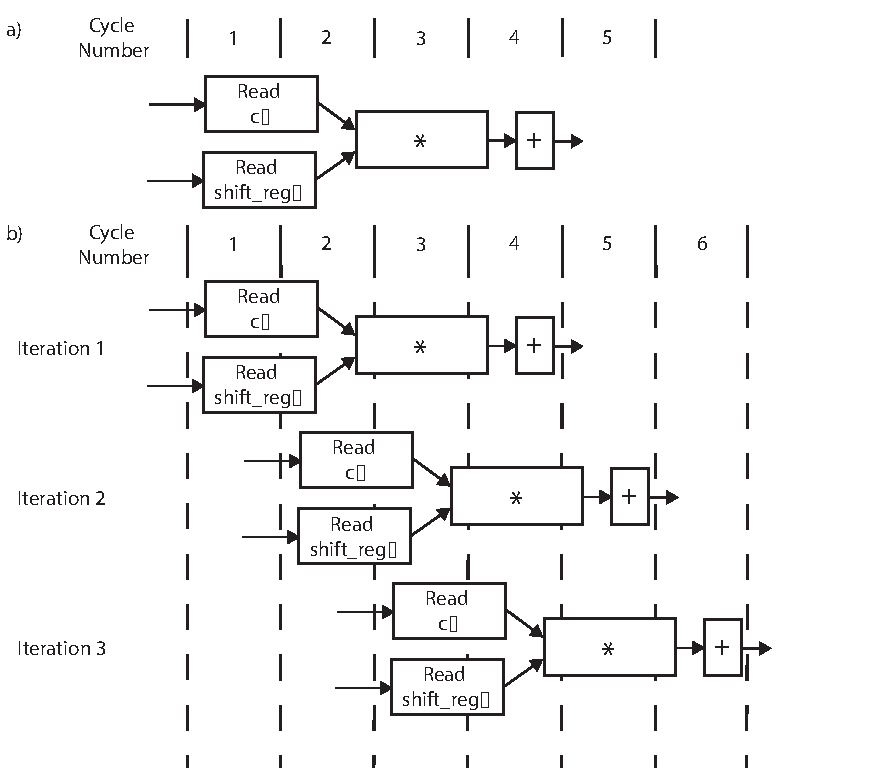
\includegraphics[width=6in]{images/pipeline_mac}
\caption{Part a) shows a schedule for the body of the \lstinline{MAC for} loop. Part b) shows the schedule for three iterations of a pipelined version of the \lstinline{MAC for} loop.}
\label{fig:pipeline_mac}
\end{figure}

There are a number of performance metrics associated with a \lstinline{for} loop. The \term{iteration latency} is the number of cycles that it takes to perform one iteration of the loop body. The iteration latency for this \lstinline{MAC for} loop is 4 cycles. The \term{\lstinline{for} loop latency} is the number of cycles required to complete the entire execution of the loop. This includes time to calculate the initialization statement (e.g., \lstinline{i = 0}), the condition statement (e.g., \lstinline{i >= 0}), and the increment statement (e.g., \lstinline{i--}). Assuming that these three header statements can be done in parallel with the loop body execution, the \VHLS tool reports the latency of this \lstinline{MAC for} loop as 44 cycles. This is the  number of iterations (11) multiplied by the iteration latency (4 cycles) plus one additional cycle to determine that the loop should stop iterating. And then you subtract one. Perhaps the only strange thing here is the ``subtract 1''. We will get to that in a second. But first, there is one additional cycle that is required at the beginning of the next iteration, which checks if the condition statement is satisfied (it is not) and then exits the loop. Now the ``subtract 1'': \VHLS determines the latency as the cycle in which the output data is ready. In this case, the final data is ready during Cycle 43. This would be written into a register at the end of Cycle 43 and correspondingly the beginning of Cycle 44.   Another way to think of this is that the latency is equal to the maximum number of registers between the input data and the output data. 

Loop pipelining is an optimization that overlaps multiple iterations of a \lstinline{for} loop. Figure \ref{fig:pipeline_mac} b) provides an example of pipelining for the \lstinline{MAC for} loop. The figure shows three iterations of the \lstinline{for} which are executed simultaneously. The first iteration is equivalent the the non-pipelined version as depicted in Figure \ref{fig:pipeline_mac} a). The difference is the start times of the subsequent iterations. In the non-pipelined version, the second iteration begins after the first iteration is completed, i.e., in Cycle 5. However, the pipelined version can start the subsequent iteration before the previous iterations complete. In the figure, Iteration 2 starts at Cycle 2, and Iteration 3 starts at Cycle 3. The remaining iterations start every consecutive cycle. Thus, the final iteration, Iteration 11, would start at Cycle 11 and it would complete during Cycle 14. Thus, the loop latency is 14.

The \term{loop initiation interval (II)} is another important performance metric. It is defined as the number of clock cycles until the next iteration of the loop can start. In our example, the loop II is 1, which means that we start a new iteration of the loop every cycle. This is graphically depicted in Figure \ref{fig:pipeline_mac} b). The II can be explicitly set using the directive. For example, the directive \lstinline{#pragma HLS pipeline II=2} informs the \VHLS tool to attempt to set the \lstinline{II=2}. Note that this may not always be possible due to resource constraints and/or dependencies in the code. The output reports will tell you exact what the \VHLS tool was able to achieve. 

\begin{exercise}
Explicitly set the loop initiation interval starting at 1 and increasing in increments of 1 cycle. How does increasing the II effect the loop latency? What are the trends?  At some point setting the II to a larger value does not make sense. What is that value in this example? How do you describe that value for a general \lstinline{for} loop?
\end{exercise}



Any \lstinline{for} loop can be pipelined, so let us now consider the \lstinline{TDL for} loop. This \lstinline{for} loop as a similar header to the \lstinline{MAC for} loop. The body of the loop performs an element by element shift of data through the array as described in Section \ref{sec:base_fir}. There are two operations: one \lstinline{Read} and one \lstinline{Write} to the \lstinline{shift_reg} array. The iteration latency of this loop is 2 cycles. The \lstinline{Read} operation takes two cycles, and the \lstinline{Write} operation is performed at the end of Cycle 2. The \lstinline{for} loop latency for this non-pipelined loop is 20 cycles.

\begin{figure}
\centering
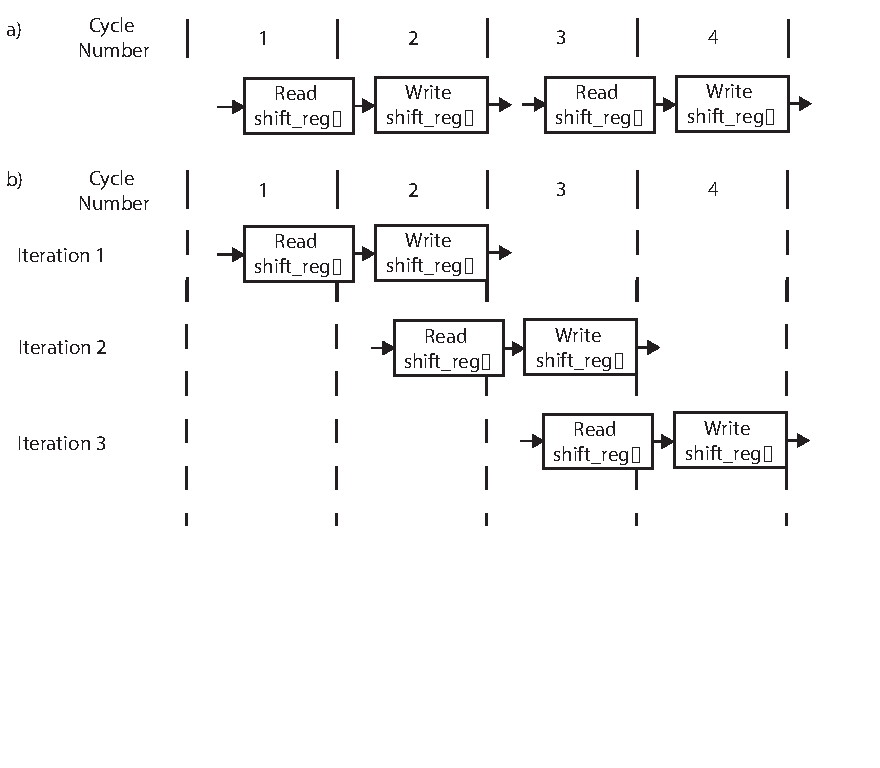
\includegraphics[width=6in]{images/pipeline_tdl}
\caption{Part a) shows a schedule for two iterations of the body of the \lstinline{TDL for} loop. Part b) shows the schedule for three iterations of a pipelined version of the \lstinline{TDL for} loop with II=1.}
\label{fig:pipeline_tdl}
\end{figure}

We can pipeline this loop by inserting the directive \lstinline{#pragma HLS pipeline II=1} after the loop header. The result of the synthesis is a loop initiation interval equal to 1 cycle.  This means that we can start a loop iteration every cycle. 

By modifying the example slightly, we can demonstrate a scenario where the resource constraints do not allow the \VHLS tool to achieve an II=1. To do this, we explicitly set the type of memory for the \lstinline{shift_reg} array. By not specifying the resource, we leave it up to the \VHLS tool to decide. But we can specify the memory using a directive, e.g., the directive \lstinline{#pragma HLS resource variable=shift_reg core=RAM_1P} forces the \VHLS tool to use a single port RAM. When using this directive in conjunction with the loop pipelining objective, the \VHLS tool will fail to pipeline this loop with an II=1. This is due to the fact that a pipelined version of this code requires both a \lstinline{Read} and \lstinline{Write} operation in the same cycle. This is not possible using a single port RAM. This is evident in Figure \ref{fig:pipeline_tdl} b). Looking at Cycle 2, we require a \lstinline{Write} operation to the array \lstinline{shift_reg} in Iteration 1, and a \lstinline{Read} operation to the same array in Iteration 2.  We can modify the directive to allow HLS more scheduling freedom by removing the explicit request for II=1, e.g. \lstinline{#pragma HLS pipeline}.  In this case, HLS will automatically increase the initiation interval until it can find a feasible schedule.

\begin{aside}
The \lstinline{RESOURCE} directive allows the user to force the \VHLS tool to map an operation to a hardware core. This can be done on arrays (as shown above) and also for variables. Consider the code \lstinline{a = b + c;}. We can use the \lstinline{RESOURCE} directive \lstinline{#pragma HLS RESOURCE variable=a core=AddSub_DSP} to tell the \VHLS tool that the \lstinline{add} operation is implemented using a DSP48. There are a wide variety of cores described in the \VHLS documentation \cite{ug902}. In general, it is advised to let the \VHLS decide the resources. If these are not satisfactory, then the designer can use directives.
\end{aside}


%\note{Talk about loop unrolling and pipelining?}



\section{Bitwidth Optimization}

The C language provides many different data types to describe different kinds of behavior.  Up until this point, we have focused on the \lstinline{int} type, which \VHLS treats as a 32-bit signed integer.   The C language also provides floating point data types, such as \lstinline{float} and \lstinline{double}, and integer data types, such as \lstinline{char}, \lstinline{short}, \lstinline{long}, and \lstinline{long long}. Integer datatypes may be \lstinline{unsigned}. All of these data types have a size which is a power of 2.

The actual number of bits for these C data types may vary depending upon the processor architecture. For example, an \lstinline{int} can be 16 bits on a micro controller and 32 bits on a general purpose processor. The C standard dictates minimum bit widths (e.g., an \lstinline{int} is at least 16 bits) and relations between the types (e.g., a \lstinline{long} is not smaller than an \lstinline{int} which is not smaller than a \lstinline{short}).  The C99 language standard eliminated this ambiguity with types such as \lstinline{int8_t}, \lstinline{int16_t}, \lstinline{int32_t}, and \lstinline{int64_t}.  

The primary benefits of using these different data types in software revolve around the amount of storage that the data type requires. For large arrays, using 8 bit values instead of 16 bit values can cut memory usage in half. The drawback is that the range of values that you can represent is reduced. An 8 bit signed value allows numbers in the range [-128,127] while the 16 bit signed data type has a range of [-32,768, 32,767].  Smaller operations may also require fewer clock cycles to execute, or may allow more instructions to be executed in parallel.

The same benefits are seen in an FPGA implementation, but they are even more pronounced. Since the \VHLS tool generates a custom data path, it will create an implementation matched to the specified data types. For example, the statement \lstinline{a = b * c} will have different latency and resource usage depending upon the data type. If all of the variables are 32 bits wide, then more primitive boolean operations need to be performed than if the variables are only 8 bits wide.   As a result, more FPGA resources (or more complex resources) must be used.  Additionally, more complex logic typically requires more pipelining in order to achieve the same frequency.  A 32-bit multiplication might require 5 internal registers to meet the same frequency that an 8 bit multiplication can achieve with only one internal register. As a result, the latency of the operation will be larger (5 cycles instead of 1 cycle) and HLS must take this into account.

\begin{exercise}
Create a simple design that implements the code \lstinline{a = b * c}. Change the data type of the variables to \lstinline{char}, \lstinline{short}, \lstinline{int}, \lstinline{long}, and \lstinline{long long}. How many cycles does the multiply operation take in each case? How many resources are used for the different data types?
\end{exercise}

\begin{exercise}
What primitive boolean operations are needed to implement the multiplication of 8-bit numbers?  How does this change when implementing multiplication of 32-bit numbers?  Hint: How many primitive decimal operations are needed to implement multiplication of two 8 digit decimal numbers? \end{exercise}

In many cases to implement optimized hardware, it is necessary to process data where the bitwidth is not a power of two. For example, analog to digital converters often output results in 10 bits, 12 bits, or 14 bits.  We could map these to 16 bit values, but this would likely reduce performance and increase resource usage.  To more accurately describe such values, \VHLS provides \term{arbitrary precision data types} which allow for signed and unsigned data types of any bitwidth. 

There are two separate classes for unsigned and signed data types:
\begin{itemize}
\item Unsigned: \lstinline{ap_uint<width>}
\item Signed: \lstinline{ap_int<width>}
\end{itemize}
where the \lstinline{width} variable is an integer between 1 and 1024\footnote{1024 is the default maximum value, and this can be changed if needed. See the \VHLS user manuals for more information on how to do this.}.  For example, \lstinline{ap_int<8>} is an 8 bit signed value (same as \lstinline{char}), and \lstinline{ap_uint<32>} is a 32 bit unsigned value (same as \lstinline{unsigned int}). This provides a more powerful data type since it can do any bitwidth, e.g., \lstinline{ap_uint<4>} or \lstinline{ap_int<537>}. To use these data types you must use C++ and include the file \lstinline{ap_int.h}, i.e., add the code \lstinline{#include "ap_int.h"} in your project and use a filename ending in `.cpp'\footnote{Similar capabilities are also available in C using the file \lstinline{ap_cint.h}}.

Consider coefficients array \lstinline{c[]} from the \lstinline{fir} filter code in Figure \ref{fig:fir11_initial}. It is reprinted here for you convenience: \lstinline|coef_t c[N] = {53, 0, -91, 0, 313, 500, 313, 0, -91, 0, 53};|. The data type \lstinline{coef_t} is defined as an \lstinline{int} meaning that we have 32 bits of precision. This is unnecessary for these constants since they range from -91 to 500. Thus we could use a smaller data type for this. We will need a signed data type since we have positive and negative values. And the maximum absolute value for any of these 11 entries is 500, which requires $\lceil \log_2 500 \rceil = 9$ bits. Since we need negative numbers, we add an additional bit. Thus \lstinline{coef_t} can be declared as \lstinline{ap_int<10>}.

\begin{exercise}
What is the appropriate data type for the variable \lstinline{i} in the \lstinline{fir} function (see Figure \ref{fig:fir11_initial})?
\end{exercise}

We can also more accurately define the data types for the other variables in the \lstinline{fir} function, e.g., \lstinline{acc} and \lstinline{shift_reg}. Consider the \lstinline{shift_reg} array first. This is storing the last 11 values of the input variable \lstinline{x}. So we know that the \lstinline{shift_reg} values can safely have the same data type as \lstinline{x}. By ``safe'', we mean that there will be no loss in precision, i.e., if \lstinline{shift_reg} had a data type with a smaller bitwidth, then some significant bits of \lstinline{x} would need to be eliminated to fit them into a value in \lstinline{shift_reg}. For example, if \lstinline{x} was defined as 16 bits (\lstinline{ap_uint<16>}) and \lstinline{shift_reg} was defined as 12 bits (\lstinline{ap_uint<12>}), then we would cut off the 4 most significant bits of \lstinline{x} when we stored it into \lstinline{shift_reg}. 

Defining the appropriate data type for \lstinline{acc} is a more difficult task. The \lstinline{acc} variable stores the multiply and accumulated sum over the \lstinline{shift_reg} and the coefficient array \lstinline{c[]} i.e., the output value of the filter. If we wish to be safe, then we calculate the largest possible value that could be stored in \lstinline{acc}, and set the bitwidth as that. 

To accomplish this, we must understand how the bitwidth increases as we perform arithmetic operations. Consider the operation \lstinline{a = b + c} where \lstinline{ap_uint<10> b} and \lstinline{ap_uint<10> c}. What is the data type for the variable \lstinline{a}? We can perform a worst case analysis here, and assume both \lstinline{a} and \lstinline{b} are the largest possible value $2^{10} = 1024$. Adding them together results in $a = 2024$ which can be represented as an 11 bit unsigned number, i.e., \lstinline{ap_uint<11>}. In general we will need one more bit than the largest bitwidth of the two number being added. That is, when  \lstinline{ap_uint<x> b} and \lstinline{ap_uint<y> c}, the data type for \lstinline{a} is \lstinline{ap_uint<z>} where $z = \max(x,y) + 1$. This same is also true when adding signed integers. 

That handles one part of the question for assigning the appropriate data type to \lstinline{acc}, but we must also deal with the multiply operation. Using the same terminology, we wish to determine the value the bitwidth $z$ given the bitwidths $x$ and $y$ (i.e., \lstinline{ap_int<z> a}, \lstinline{ap_int<x> b}, \lstinline{ap_int<y> c}) for the operation \lstinline{a = b * c}. While we will not go into the details, the formula is $z = x + y$. 

\begin{exercise}
Given these two formulas, determine the bitwidth of \lstinline{acc} such that it is safe.
\end{exercise}

Ultimately we are storing \lstinline{acc} into the variable \lstinline{y} which is an output port of the function. Therefore, if the bitwidth of \lstinline{acc} is larger than the bitwidth of \lstinline{c}, the value in \lstinline{acc} will be truncated to be stored into \lstinline{y}. Thus, is it even important to insure that the bitwidth of \lstinline{acc} is large enough so that it can handle the full precision of the multiply and accumulate operations? 

The answer to the question lies in the tolerance of the application. In many digital signal processing applications, the data itself is noisy, meaning that the lower several bits may not have any significance. In addition, in signal processing applications, we often perform numerical approximations when processing data which can introduce additional error. Thus, it may not be important that we insure that the \lstinline{acc} variable has enough precision to return a completely precise result.  On the other hand, it may be desirable to keep more bits in the accumulation and then round the final answer again to reduce the overall rounding error in the computation. Other applications, such as scientific computing, more dynamic range is often required, which may lead to the use of floating point numbers instead of integer or fixed-point arithmetic. So what is the correct answer? Ultimately it is up to the tolerance of the application designer.


%\section{Shift and Add}
%\note{Not sure if this is necessary. It is a good implementation, but it doesn't really highlight anything important about HLS.}

\section{Complex FIR Filter}

%\note{Describe how you can make functions and use the real FIR to create a complex FIR using two instances of the real FIR. Use to motivate hierarchical design.}

To this point, we have solely looked at filtering real numbers. Many digital wireless communication systems deal with complex numbers using in-phase (I) and quadrature (Q) components. Fortunately, it is possible to create a complex FIR filter using real FIR filter as we describe in the following.

To understand how to build a complex FIR filter from real FIR filters consider Equation \ref{eq:complex_fir}. Assume that $(I_{in}, Q_{in})$ is one sample of the input data that we wish to filter.  And one of the complex FIR filter coefficients is denoted as $(I_{fir}, Q_{fir})$. There will be more than one input sample and complex coefficient, but let us not worry about that for now.

\begin{equation}
(I_{in} + j  Q_{in})(I_{fir} + j  Q_{fir}) = (I_{in} I_{fir} - Q_{in}  Q_{fir}) + j  (Q_{in}  I_{fir} + I_{in} Q_{fir})
\label{eq:complex_fir}
\end{equation}

Equation \ref{eq:complex_fir} shows the multiplication of the input complex number by one coefficient of the complex FIR filter. The right side of the equation shows that the real portion of the output of complex input filtered by a complex FIR filter is $I_{in} I_{fir} - Q_{in}  Q_{fir}$ and the imaginary output is $Q_{in}  I_{fir} + I_{in} Q_{fir}$. This implies that we can separate the complex FIR filter operation into four real filters as shown in Figure \ref{fig:complex_fir}.

\begin{figure}
\centering
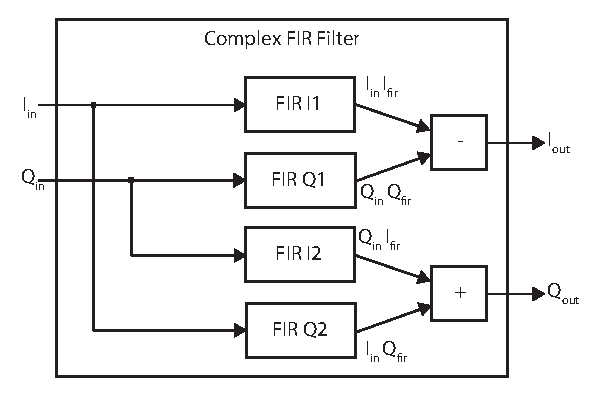
\includegraphics[width=6in]{images/complex_fir}
\caption{A complex FIR filter built from four real FIR filters. The input I and Q samples are feed into four different real FIR filters. The FIR filters hold the in-phase (FIR I) and quadrature (FIR Q) complex coefficients. }
\label{fig:complex_fir}
\end{figure}

A complex FIR filter takes as input a complex number $(I_{in},Q_{in})$ and outputs a complex filtered value $(I_{out},Q_{out})$. Figure \ref{fig:complex_fir} provides a block diagram of this complex filter using four real FIR filters (FIR I1, FIR Q1, FIR I2, FIR Q2). The filters FIR I1 and FIR I2 are equivalent, i.e., they have the exact same coefficients. FIR Q1 and FIR Q2 are also equivalent. The output of each of these filters corresponds to a term from Equation \ref{eq:complex_fir}. These output are then added or subtracted to provide the final filtered complex output $(I_{out}, Q_{out})$. 

We used a hierarchical structure to define this complex FIR filter. \VHLS implements hierarchy using functions. Taking the previous real FIR function \lstinline{void fir (data_t *y, data_t x)} we can create another function that encapsulates four versions of this \lstinline{fir} function to create the complex FIR filter. This code is shown in Figure \ref{fig:complex_fir_code}.

\begin{figure}
\lstinputlisting{examples/complex_fir.cpp}
\caption{The \VHLS code to hierarchically implement a complex FIR filter using four real FIR filters.}
\label{fig:complex_fir_code}
\end{figure}

The code defines four functions \lstinline{firI1}, \lstinline{firQ1}, \lstinline{firI2}, and \lstinline{firQ2}. Each of these functions has the exact same code, e.g., that of the \lstinline{fir} function from Figure \ref{fig:fir11_initial}. Typically, we would not need to replicate the function; we could simply call the same function four times. However, this is not possible in this case due to the \lstinline{static} keyword used within the \lstinline{fir} function for the \lstinline{shift_reg}. \note{A good solution to this is to convert the function to a class.}

The function calls act as interfaces. The \VHLS tool does not optimize across function boundaries. That is, each \lstinline{fir} function synthesized independently, and treated more or less as a black box in the \lstinline{complexFIR} function. You can use the \lstinline{inline} directive if you want the \VHLS tool to co-optimize a particular function within its parent function. This will add the code from that function into the parent function and eliminate the hierarchical structure. While this can increase the potential for benefits in performance and area, it also creates a large amount of code that the tool must synthesize. That may take a long time, even fail to synthesize, or may result in a non-optimal design. Therefore, use the \lstinline{inline} directive carefully. Also note that the \VHLS tool may choose to inline functions on its own. These are typically functions with a small amount of code.

\begin{figure}
\lstinputlisting{examples/inline.c}
\caption{ A simple and trivial example to demonstrate the \lstinline{inline} directive. The \lstinline{top_function} has four function calls to the function \lstinline{mul}. If we placed an \lstinline{inline} directive on the \lstinline{mul} function, the result is similar to what you see in the function \lstinline{inlined_top_function}. }
\label{fig:inline}
\end{figure}

\begin{aside}
The \lstinline{inline} directive removes function boundaries, which may enable additional opportunities for the \VHLS tool at the cost of increasing the complexity of the synthesis problem, i.e., it will likely make the synthesis time longer.  It also eliminates any overhead associated with performing the function call. It allows for different implementations while maintaining the structure of the code, and making it hierarchical and more readable.

The code in Figure \ref{fig:inline} provides an example of how the inline directive works. The function \lstinline{inlined_top_function} is the result of using the \lstinline{inline} directive on the \lstinline{mul} function.

The \VHLS tool will sometimes choose to inline functions automatically. For example, it will very likely choose to inline the \lstinline{mul} function from Figure \ref{fig:inline} since it is small. You can force the tool to keep the function hierarchy by placing an \lstinline{inline} directive in the function with the \lstinline{off} argument.

The \lstinline{inline} directive also has a \lstinline{recursive} argument that inlines all functions called within the inlined function to also be inlined. That is, it will recursively add the code into the parent functions from every child function. This could create a substantial code base, so use this function carefully.

An inlined function will not have separate entries in the report since all of the logic will be associated with the parent function.
\end{aside}

%\note{Talk a bit about Interface Synthesis here?}

\section{Conclusion}
This chapter describes the specification and optimization of a FIR filter using the \VHLS tool. The goal is to provide an overview of the HLS process. The first step in this process is understanding the basic concepts behind the computation of the FIR filter. This does not require a deep mathematical understanding, but certainly enough knowledge to write it in a manner that is synthesizable by the \VHLS tool. This may require translating the code from a different language (e.g., MATLAB, Java, C++, Python, etc.). Many times it requires rewriting to use simpler data structures, e.g., one that is explicitly implemented in an array. And it often involves removing system calls and other code not supported by the HLS tool. 

Creating an optimum architecture requires a basic understanding about how the HLS tool performs its synthesis and optimization process to RTL code. It is certainly not unnecessary to understand the exact HLS algorithms for schedule, binding, resource allocation, etc. (and many times these are proprietary). But having a general idea of the process does aid the designer in writing code that maps well to hardware. Throughout the chapter, we talked about some of the key features of the HLS synthesis process that are necessary to understand when performing various optimizations. It is especially important to understand the way that the HLS tool reports performance, which we describe in Chapter \ref{sec:fir-performance}. 

Additionally, we presented some basic HLS optimizations (including loop and bitwidth optimizations). We highlighted their benefits and potential drawbacks using the FIR filter as an example. These are common optimizations that can be applied across a wide range of applications. We provide more details about these optimizations in subsequent chapters as we walk through the implementation of other more complex applications. 

%Finally, there is an entire project devoted to further optimizing the FIR filter. This is located in the Appendix in Chapter \ref{chapter:FIR_Project}. 